\documentclass{article}

\usepackage[utf8]{inputenc}
\usepackage[T1]{fontenc}
\usepackage{geometry}
\usepackage{graphicx}
\usepackage{subcaption}
\usepackage{verbatim}
\usepackage{amsmath,amssymb}
\usepackage[section]{placeins}
\usepackage{amstext}
\usepackage{enumitem} %PERMETTE L'USO DI ELENCHI NUMERATI


\geometry{a4paper}

\usepackage[french,italian,english]{babel}
\frenchspacing

\title{Relazione dell'esperimento di Millikan}
\author{Lorenzo Ramella, Alessandro Matteo Rossi, Marco Tambini}
\date{27 novembre 2020}

\begin{document}
\maketitle

\begingroup
\selectlanguage{english}
\begin{abstract}
L’esperimento si propone di fornire una stima della carica dell’elettrone. La carica viene studiata partendo dallo studio del moto di alcune goccioline d’olio elettricamente cariche in presenza ed in assenza di un campo elettrico. L'esperienza è stata svolta da due studenti in due turni separati di laboratorio.


\vspace{4mm}

Durante il primo turno di laboratorio, Lorenzo Ramella ed un altro studente (Giovanna Scaiano, appartenente ad un diverso gruppo), hanno studiato il moto di 10 goccioline d’olio cariche. 

\vspace{4mm}

Durante il secondo turno di laboratorio, Alessandro Matteo Rossi ed un altro studente (Alessandro Rossi [sic], appartenente ad un diverso gruppo), hanno studiato il moto di 13 goccioline d’olio cariche. 

\vspace{4mm}

I dati ottenuti sono stati uniti e da questi si è potuti giungere ad una stima della carica dell'elettrone.

\[q_e = - 1,59 \cdot\ 10^{-19} \pm 4 \cdot 10^{-21} \, \textrm{C}\]

\end{abstract}
\endgroup

\selectlanguage{italian}
\tableofcontents

\section{Introduzione teorica}
L'esperimento si propone di misurare la carica dell'elettrone partendo dallo studio del moto di microscopiche goccioline d'olio elettrizzate. La misura richiede di misurare la velocità limite delle goccioline d'olio in presenza ed in assenza di un campo elettrico. Assumendo che le goccioline siano di forma approssimativamente sferica e che l'asse $z$ sia rivolto verso il basso, si possono scrivere le seguenti equazioni:

In assenza di campo elettrico:

\begin{equation}
(4 \pi /3)r^3 (\rho _o - \rho _a)g - 6\pi \eta r v_0=0 
\end{equation}

Dove $\rho _o$ e $\rho _a$ sono le densità rispettivamente dell'olio e dell'aria, $r$ è il raggio della gocciolina, $g$ è l'accelerazione di gravità, $\eta$ la viscosità dell'aria e $v_0$ la velocià limite in assenza di campo elettrico. Il primo addendo è la forza di gravità che agisce sulla gocciolina (a cui è già stata tolta la forza di Archimede), mentre il secondo è la forza di attrito viscoso che agisce sulla gocciolina; il segno meno indica che l'attrito si oppone al moto.

In presenza di campo elettrico:

\begin{equation}
(4 \pi /3)r^3 (\rho _o - \rho _a)g - 6\pi \eta r v + QE=0 
\end{equation}

Dove $v$ è la nuova velocità limite.

Si possono combinare queste due relazioni per eliminare il termine $\eta$ 

\[6\pi \eta r=\frac{(4 \pi /3)r^3 (\rho _o - \rho _a)g}{v_0}=\frac{(4 \pi /3)r^3 (\rho _o - \rho _a)g + QE}{v}\]
\[-QE=(4 \pi /3)r^3(\rho _o - \rho _a)g - \frac{v(4 \pi /3)r^3(\rho _o - \rho _a)g}{v_0}\]

\begin{equation}
Q=-(4 \pi /3)r^3(\rho _o - \rho _a)(g/E)(1-v/v_0)
\end{equation}

Conviene ora trattare separatamente il caso in cui la gocciolina salga e quella in cui scenda, in modo da preoccuparci solo del modulo della velocità in fase di presa dati:

\begin{equation}
Q=-(4 \pi /3)r^3(\rho _o - \rho _a)(g/E)(1 - |v|/v_0) \quad \textrm{per} \quad v>0 \quad (v \downarrow)
\end{equation}

\begin{equation}
Q=-(4 \pi /3)r^3(\rho _o - \rho _a)(g/E)(1+|v|/v_0) \quad \textrm{per} \quad v<0 \quad (v \uparrow)
\end{equation}

Tutte le quantità contenute in queste espressioni sono note o facilmente misurabili, eccetto per $\eta$. Essendo infatti il raggio delle goccioline tanto piccolo da essere dello stesso ordine di grandezza del libero cammino medio delle molecole d'aria, la viscosità effettiva dell'aria non dipende solo dalle condizioni di pressione e temperatura ma anche dal raggio della gocciolina stessa. Empiricamente è stato mostrato che 

\begin{equation}
\eta _{e\!f\!f} =\frac{\eta}{1+\frac{b}{pr}}
\end{equation}

\begin{equation}
\eta (N s/m^2) =[1.800+(t-15)\cdot 4.765 \cdot10^{-3}]\cdot 10^{-5}
\end{equation}

dove $t$ è la temperatura (in gradi centigradi), $p$ la pressione dell'aria (in Pascal) e $b$ una costante che per l'aria vale $b=8.2\cdot10^{-3} \,Pa\:m$. Possiamo quindi esprimere il raggio della gocciolina d'olio come

\begin{equation}
r=\sqrt{\left( \frac{b}{2p} \right)^2 + \frac{9\eta v_0}{2g(\rho _o - \rho _a)}}-\frac{b}{2p}
\label{raggio}
\end{equation}

Una volta trovati i valori di carica di un numero possibilmente grande di goccioline d'olio, possiamo procedere ricordando che la carica è quantizzata, ovvero che la carica di una gocciolina d'olio è pari a $nq$, dove $n$ è un numero razionale e $q$ è la carica dell'elettrone. Definiamo la funzione $k_i (Q_i, q)$ come l'intero più vicino al rapporto $\frac{Q_i}{q}$ (ovvero la parte intera di $\frac{Q_i}{q}+0.5$). Ci aspettiamo che $Q_i = qk_i$. Possiamo quindi usare Excel, o un programma appositamente scritto, per "tentare" diversi possibili valori di q e per ognuno valutare la funzione

\begin{equation}
S(q)=\sum_{i=1}^{N}{\left( \frac{Q_i}{k_i} - q \right)^2}
\label{Anal1}
\end{equation}

corrispondente allo scarto quadratico medio tra i valori misurati $\frac{Q_i}{k_i}$ e il valore atteso $q$. Il punto di minimo $q_c$ di questa funzione corrisponde al valore più probabile da attribuire a $q$. Una volta localizzato l'intorno in cui è localizzato il minimo si può imporre la derivata di $S(q)$ uguale a zero e ottenere 

\begin{equation}
q_e=\frac{1}{N} \sum_{i=1}^{N}{\frac{Q_i}{k_i(Q_i,q_c)}}
\label{Anal2}
\end{equation}

Ovvero la media delle quantità $\frac{Q_i}{k_i(Q_i,q_c)}$. Come incertezza $\sigma _q$ si può prendere la deviazione standard della media.

\pagebreak
\section{Progettazione dell'esperimento}

\begin{figure}[h]
\centering
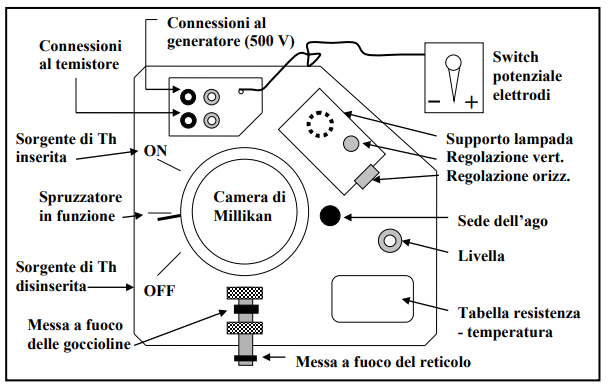
\includegraphics[scale=0.7]{SchemaMillikan1}
\caption{Schema dell'apparato sperimentale visto dall'alto}
\end{figure}

\begin{figure}[h!]
\centering
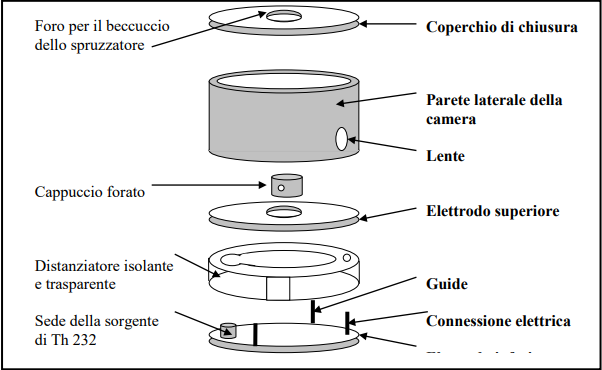
\includegraphics[scale=0.7]{SchemaMillikan2}
\caption{Schema dei componenti della camera di Millikan}
\end{figure}

L'apparto si compone di un piano orizzontale su cui è montata la camera di Millikan, con una lampada che ne illumina l'interno e un microscopio che permette di vedere le gocce. Il microscopio è dotato di un reticolo a quadretti di lato 0,5 mm, per misurare il moto delle gocce. Per avere un riferimento più preciso è presente anche una quadrettatura più fine, con quadretti di lato 0,1mm. La camera si compone di due elettrodi (che vengono connessi al generatore di tensione) separati da un distanziale trasparente (che permette quindi alla lampada di illuminare le gocce e allo sperimentatore di vederle). Un cappuccio forato, posto in un foro nell'elettrodo superiore, permette di "filtrare" le gocce che entrano nella camera. La struttura è completata da una parete laterale e da un coperchio, nel quale è stato praticato un foro nel quale spruzzare le goccioline. Alla base della camera c'è poi una sorgente di Torio (Th 232), attivabile a discrezione dello sperimentatore per caricare ulteriormente le gocce.

\vspace{5mm}

Lo sperimentatore ha a dispozione anche uno spruzzatore, dotato di un beccuccio uncinato per spruzzare le gocce nella camera dal foro superiore. Le gocce, uscendo dallo spruzzatore, vengono caricate per strofinio.

\vspace{5mm}

Dopo aver disinfettato con cura tutti i componenti dell'apparato sperimentale, è stato verificato che il piano fosse in posizione orizzontale usando la livella. Usando un micrometro (sensibilità del centesimo di millimetro), è stato misurato lo spessore del distanziale isolante e abbiamo montato la camera di Millikan (eccetto per il cappuccio forato e il coperchio).

\begin{figure}[h]
\centering
\includegraphics[width=0.7\linewidth]{FotoMillikan1}
\caption{Foto della messa a fuoco dell'ago}
\end{figure}

A questo punto è stata fatta la messa a fuoco dell'ago, inserito nella camera, avendo cura di mettere a fuoco sia il reticolo che lo stesso ago. Questa fase di messa fuoco è fondamentale per poter poi successivamente vedere bene le gocce. Una volta completata la messa a fuoco è stato rimosso l'ago, riponendolo con cura nella sua sede, ed è stato completato l'assemblamento della camera.

\begin{figure}[h]
  \centering
  \begin{subfigure}[b]{0.4\linewidth}
    \includegraphics[width=\linewidth]{FotoMillikan2}
    \caption{Foto del generatore di tensione}
  \end{subfigure}
  \begin{subfigure}[b]{0.4\linewidth}
    \includegraphics[width=\linewidth]{FotoMillikan3}
    \caption{Foto del termistore}
  \end{subfigure}
  \caption{Foto del generatore di tensione e del termistore}
\end{figure}

\begin{figure}[h!]
\centering
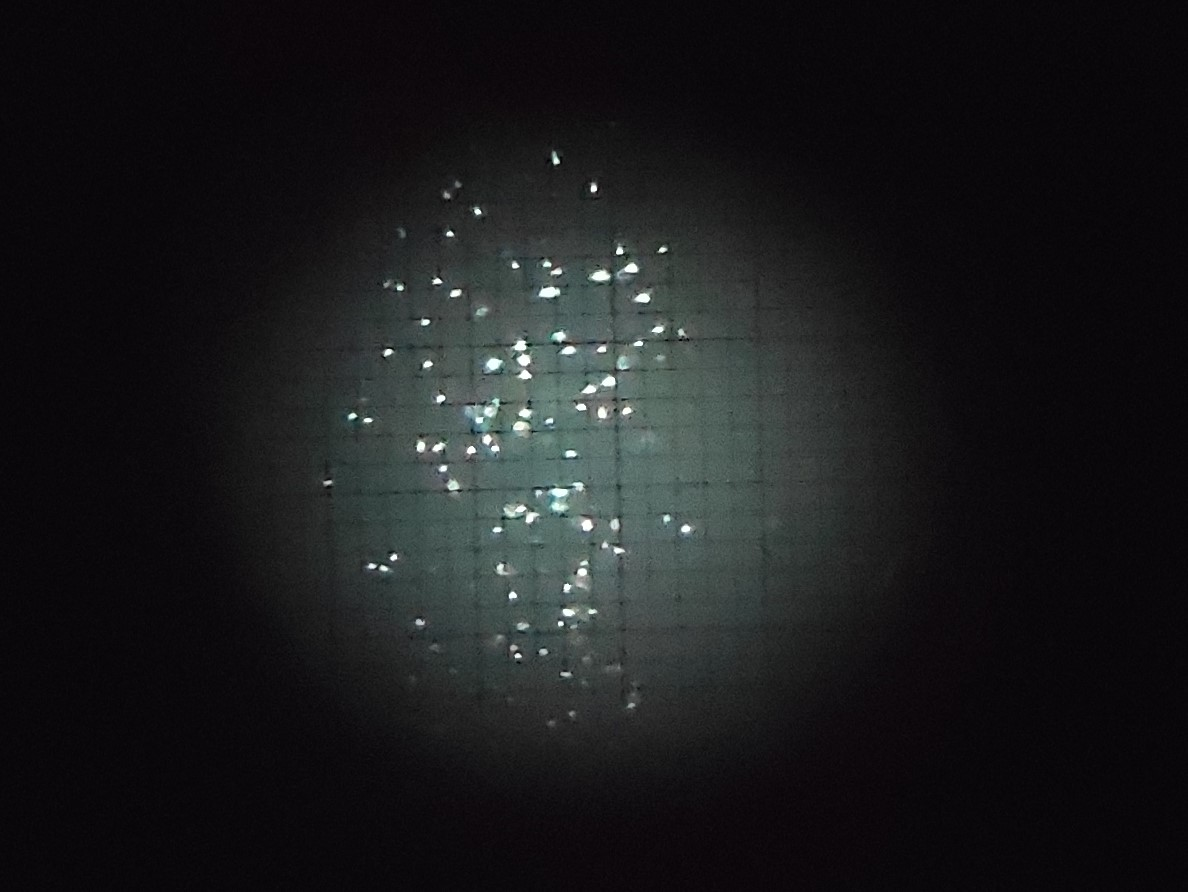
\includegraphics[width=0.6\linewidth]{FotoMillikan4}
\caption{Foto di alcune gocce ''di prova'', spruzzate nella camera. Ben visibile il reticolo}
\end{figure}

\vspace{5mm}

È stato quindi connesso il generatore di tensione (regolandolo alla tensione di 400V) e il termistore. Il termistore è uno strumento che, collegato anch'esso agli elettrodi, permette di misurare la resistenza elettrica all'interno della camera. I dati riportati nella tabella \ref{TabRes} permettono di conoscere il valore della temperatura nella camera in funzione della resistenza misurata.

\begin{table}[h!]
\centering
\begin{tabular}{ || c | c || c | c || c | c || c | c || c | c || }
  \hline
  $t (\textrm{C})$ & $R (\textrm{M} \Omega)$ & $t (\textrm{C})$ & $R (\textrm{M} \Omega)$ & $t (\textrm{C})$ & $R (\textrm{M} \Omega)$ & $t (\textrm{C})$ & $R (\textrm{M} \Omega)$ & $t (\textrm{C})$ & $R (\textrm{M} \Omega)$ \\
  \hline
  \hline
  $10$ & $3.239$ & $15$ & $2.700$ & $20$ & $2.300$ & $25$ & $2.000$ & $30$ & $1.774$ \\
  $11$ & $3.118$ & $16$ & $2.610$ & $21$ & $2.233$ & $26$ & $1.950$ & $31$ & $1.736$ \\
  $12$ & $3.004$ & $17$ & $2.526$ & $22$ & $2.169$ & $27$ & $1.902$ & $32$ & $1.700$ \\
  $13$ & $2.897$ & $18$ & $2.446$ & $23$ & $2.110$ & $28$ & $1.857$ & $33$ & $1.666$ \\
  $14$ & $2.795$ & $19$ & $2.371$ & $24$ & $2.053$ & $29$ & $1.815$ & $34$ & $1.634$ \\
  \hline
\end{tabular}
  \caption{Resistenza elettrica del termistore in funzione della temperatura}
  \label{TabRes}
\end{table}

\begin{table}[h!]
\centering
\begin{tabular}{ | c | c | c | c | c | }
  \hline
  $p$ (Pa) & $g (\frac{\textrm{m}}{\textrm{s}^2})$ & $\rho _o (\frac{\textrm{kg}}{\textrm{m}^3})$ & $\rho _a (\frac{\textrm{kg}}{\textrm{m}^3})$ & $b$ (Pa m) \\
  \hline
  $1 \cdot 10^6$ & $9,806$ & $860$ & $1,29$ & $0,0082$ \\
  \hline
\end{tabular}
  \caption{Costanti note}
  \label{TabCos}
\end{table}

\pagebreak

\section{Misure gocce 1-10}

Le misure relative alle prime dieci gocce sono state raccolte nel corso del primo turno di laboratorio. Di ogni goccia è stata misurata la velocità in caduta libera, in salita con il campo elettrico e in caduta con il campo elettrico. In ognuno di questi movimenti è stato misurato il tempo necessario per percorrere uno spazio di quattro quadretti, misurando anche gli intertempi relativi ad ogni quadretto. Questa misura è stata realizzata utilizando il cronometro preinstallato negli smartphone degli sperimentatori.

\vspace{3mm}

Per ogni goccia sono stati inoltre controllati, prima di effettuare le misure di velocità, i valori di resistenza e differenza di potenziale segnati rispettivamente sul termistore e sul generatore. Il valore della temperatura è stato stimato con un'interpolazione lineare con i valori tabulati, ed è stata data al valore ottenuto un'incertezza di 1° C.

\vspace{3mm}

Le misure relative alle prime 5 gocce sono state eseguite da Scaiano che, osservando nel microscopio, segnalava a Ramella quando fermare il cronometro. Per le successive 5 gocce, i due studenti si sono invertiti. Come incertezza per i tempi abbiamo deciso di usare 0,5 s, una stima conservativa dei riflessi umani.

\vspace{3mm}

Per ogni misura di tempo in caduta libera $\Delta t$ abbiamo calcolato la velocità $v_r = \frac{\Delta z}{\Delta t}$ (con relativa incertezza $\sigma v = \sqrt{(\frac{\sigma \Delta z}{\Delta t})^2 + (\frac{\Delta z}{\Delta t^2}\sigma \Delta t)^2}$ dove $\Delta z = 0,5 mm$ e $ \sigma\Delta z = 0,1 mm$) e il raggio (vedi Formula (\ref{raggio})). L'incertezza del raggio, calcolata con la formula della propagazione degli errori, è

\[\sigma r = \sqrt{\left( \frac{9 \eta \cdot \sigma v}{4g(\rho_o - \rho_a)\sqrt{(\frac{b}{2p})^2+\frac{9v\eta}{2g(\rho_o - \rho_a)}}}\right)^2 + \left( \frac{9v \cdot \sigma \eta}{4g(\rho_o - \rho_a)\sqrt{(\frac{b}{2p})^2+\frac{9v\eta}{2g(\rho_o - \rho_a)}}}\right)^2} \]

\[\textrm{dove} \quad \sigma \eta = 4,765 \cdot 10^{-8} \cdot T \cdot \sigma T\]

La nostra miglior stima del raggio è la media pesata tra i quattro valori del raggio così misurati.

\vspace{4mm}

Poiché noi siamo interessati solo al valore assoluto della carica e non al suo segno, abbiamo trascurato il segno del campo elettrico nel calcolo della carica $Q$. Di conseguenza, d'ora in poi useremo il termine $Q$ per riferirci al valore assoluto della carica misurata:

\[Q=(4 \pi /3)r^3(\rho _o - \rho _a)(g/|E|)(1 \pm |v|/v_0)\]

\[ \textrm{dove} \quad |E|=\frac{|\Delta V|}{d}\]

Per ogni misura di tempo in presenza del campo elettrico $\Delta t$ abbiamo calcolato la velocità $v_e = \frac{\Delta z}{\Delta t}$ e, da questa, la carica Q. La miglior stima di $v_0$ è la media pesata tra le velocità $v_r$ precedentemente ricavate.

\vspace{3mm}

Problemi tecnici riscontrati: tutte le dieci misure si sono svolte usando lo stesso apparato sperimentale, a causa di un malfunzionamento di uno dei due apparati a disposizione. L’interruttore dell’apparato su cui è stato svolto l’esperimento era malfunzionante, ed è stato sostituito prima dell’inizio dell’esperienza. I due studenti si sono alternati usando lo stesso apparato, disinfettandolo con cura ad ogni cambio.

\pagebreak

\subsection{Misura distanziale}

Sono state effettuate 5 misure dello spessore del distanziale

\begin{table}[h!]
\centering
\begin{tabular}{ | c | c | c | }
  \hline
  $\#$ & d (mm) & $\sigma$d (mm) \\
  \hline
  $1$ & $7,59$ & $0,01$ \\
  $2$ & $7,59$ & $0,01$ \\
  $3$ & $7,59$ & $0,01$ \\
  $4$ & $7,59$ & $0,01$ \\
  $5$ & $7,57$ & $0,01$ \\
  \hline
  & media & $\sigma$media \\
  \hline
  & $7,59$ & $0,01$ \\
  \hline
\end{tabular}
  \caption{Misura del distanziale}
  \label{dist_1}
\end{table}

come incertezza della media si è scelto di usare la sensibilità del micrometro.

\subsection{Misura delle gocce}

Goccia 1:

\begin{figure}[h]
\centering
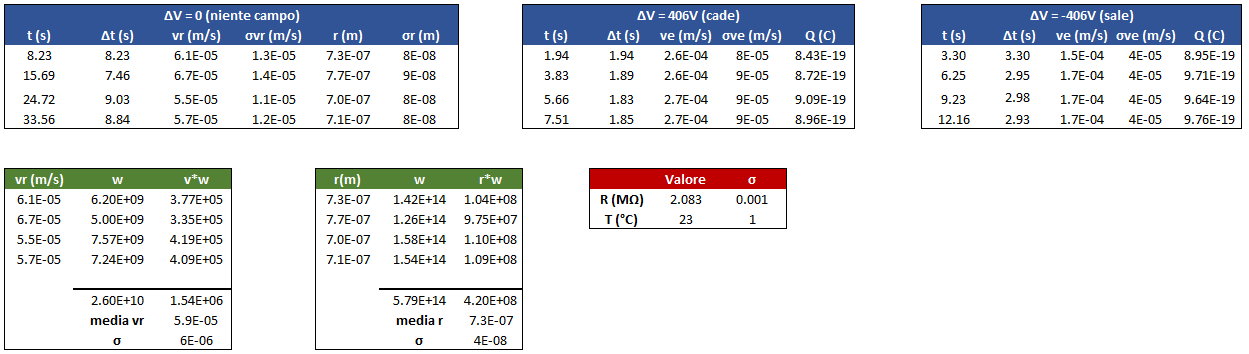
\includegraphics[width=\linewidth]{Goccia1}
\end{figure}

\vspace{10mm}

Goccia 2:

\begin{figure}[h]
\centering
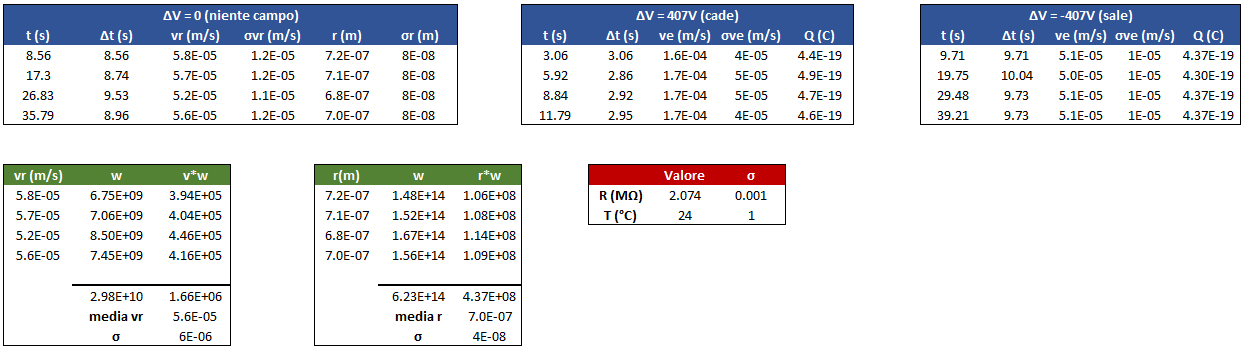
\includegraphics[width=\linewidth]{Goccia2}
\end{figure}

\pagebreak

Goccia 3:

\begin{figure}[h]
\centering
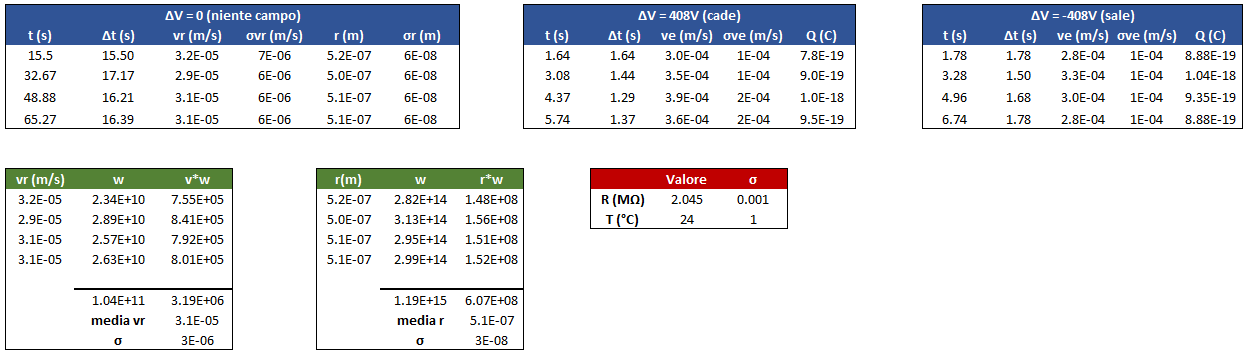
\includegraphics[width=\linewidth]{Goccia3}
\end{figure}

\vspace{10mm}

Goccia 4:

\begin{figure}[h]
\centering
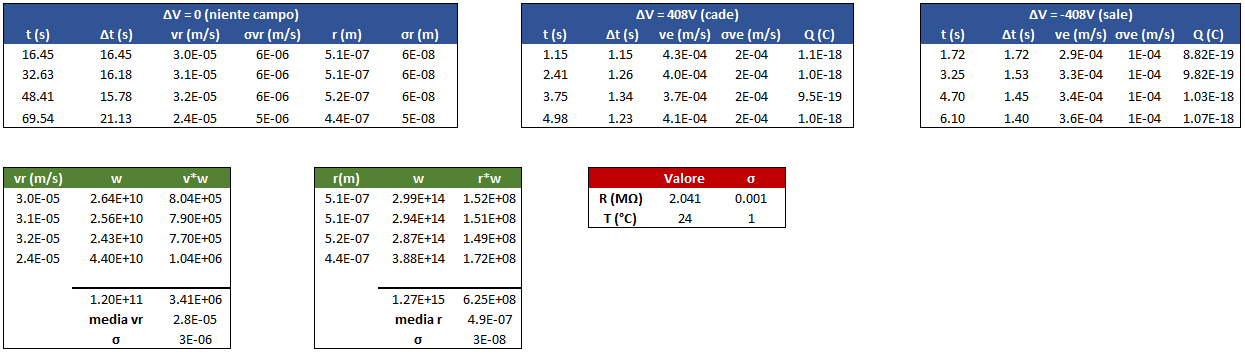
\includegraphics[width=\linewidth]{Goccia4}
\end{figure}

\vspace{10mm}

Goccia 5:

\begin{figure}[h]
\centering
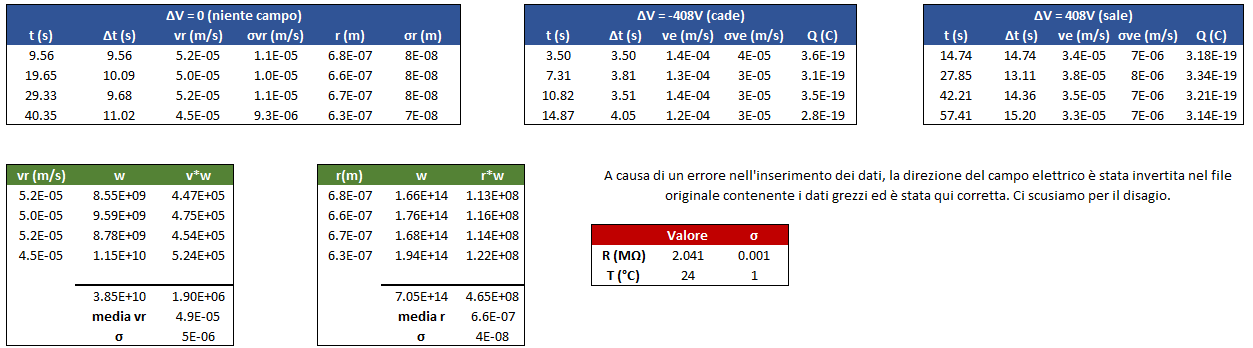
\includegraphics[width=\linewidth]{Goccia5}
\end{figure}

\pagebreak

Goccia 6:

\begin{figure}[h]
\centering
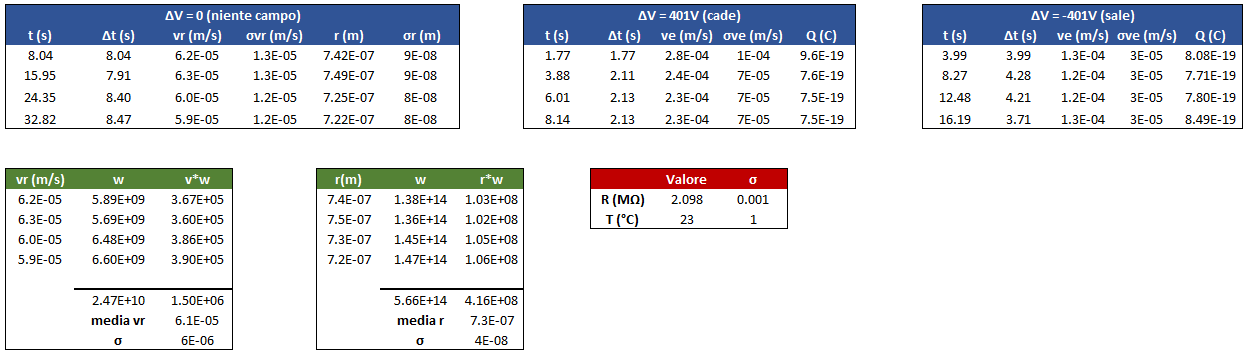
\includegraphics[width=\linewidth]{Goccia6}
\end{figure}

\vspace{10mm}

Goccia 7:

\begin{figure}[h]
\centering
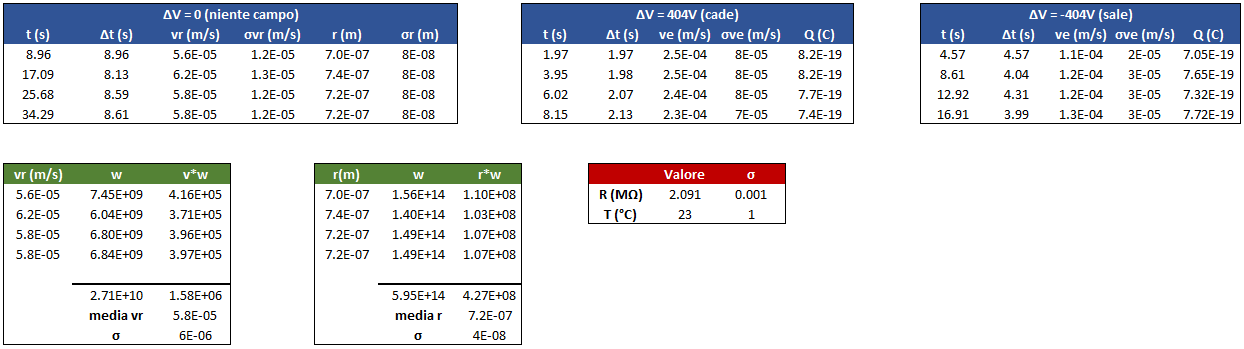
\includegraphics[width=\linewidth]{Goccia7}
\end{figure}

\vspace{10mm}

Goccia 8:

\begin{figure}[h]
\centering
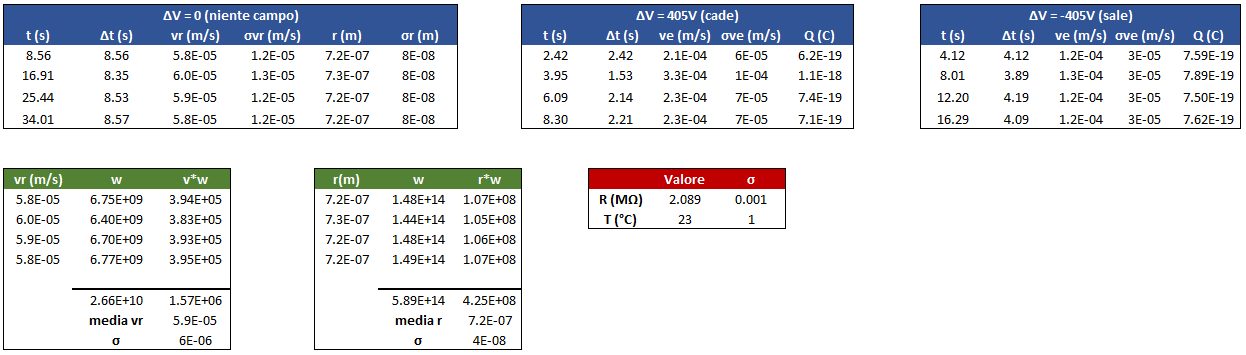
\includegraphics[width=\linewidth]{Goccia8}
\end{figure}

\pagebreak

Goccia 9:

\begin{figure}[h]
\centering
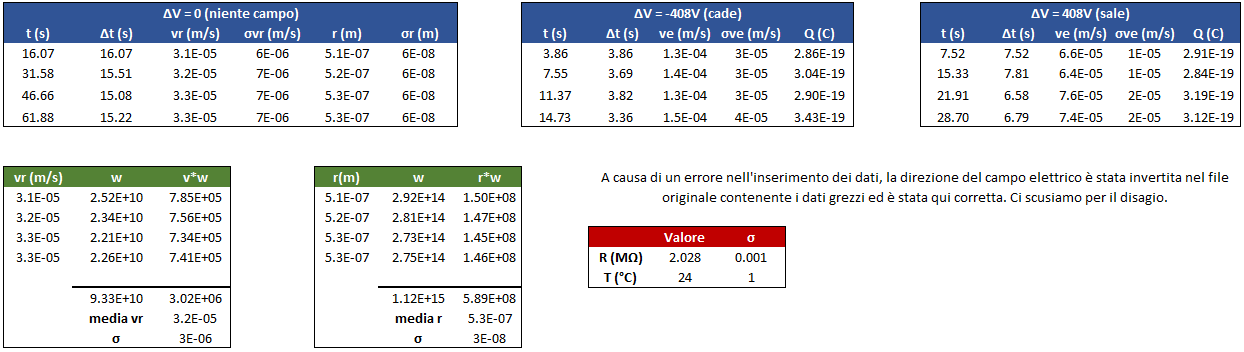
\includegraphics[width=\linewidth]{Goccia9}
\end{figure}

\vspace{10mm}

Goccia 10:

\begin{figure}[h]
\centering
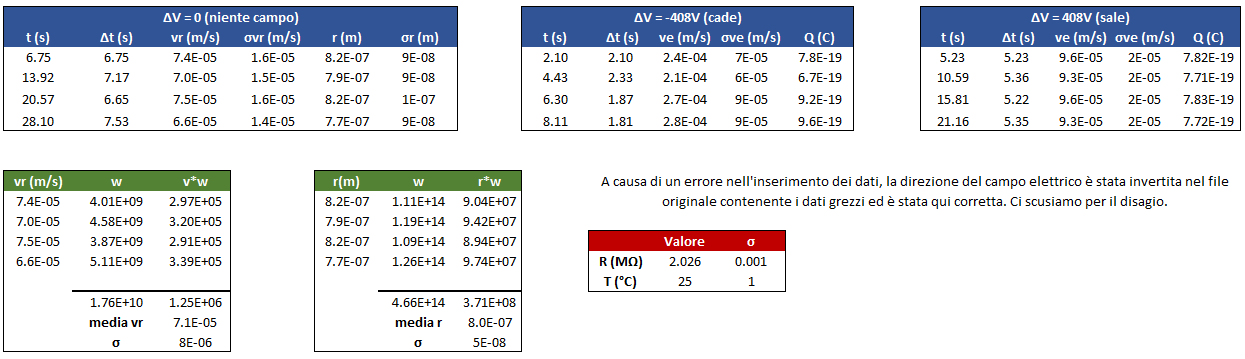
\includegraphics[width=\linewidth]{Goccia10}
\end{figure}

\subsection{Confronto raggi}

\begin{figure}[h]
\centering
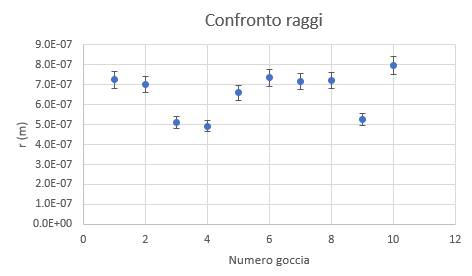
\includegraphics[width=0.6\linewidth]{Confronto_r_1}
\end{figure}

Le diverse gocce usate nell'esperimento hanno tutte raggi di dimensioni simili, ovvero dello stesso ordine di grandezza. Possiamo escludere l'eventualità di gravi errori nella presa dati.

Le dimensioni delle gocce sono tali da escludere effetti significativi di moti browniani.

\section{Misure gocce 11-19}

I metodi e le analisi utilizzate nel secondo turno di laboratorio sono analoghe a quelle indicate per il primo. Le gocce trattate in questa sezione sono state misurate con l'apparato in dotazione a Alessandro Matteo Rossi, che dava i tempi ad Alessandro Rossi.

\vspace{5mm}

Problemi tecnici riscontrati: a causa della bassa responsività delle gocce, è stato fatto pesante uso della sorgente di Torio, che ha portato a gocce molto cariche. 

\subsection{Misura distanziale}

Sono state effettuate 5 misure dello spessore del distanziale

\begin{table}[h!]
\centering
\begin{tabular}{ | c | c | c | }
  \hline
  $\#$ & d (mm) & $\sigma$d (mm) \\
  \hline
  $1$ & $7,62$ & $0,01$ \\
  $2$ & $7,63$ & $0,01$ \\
  $3$ & $7,63$ & $0,01$ \\
  $4$ & $7,63$ & $0,01$ \\
  $5$ & $7,63$ & $0,01$ \\
  \hline
  & media & $\sigma$media \\
  \hline
  & $7,63$ & $0,01$ \\
  \hline
\end{tabular}
  \caption{Misura del distanziale}
  \label{dist_2}
\end{table}

come incertezza della media si è scelto di usare la sensibilità del micrometro.

\subsection{Misura delle gocce}

Goccia 11:

\begin{figure}[h]
\centering
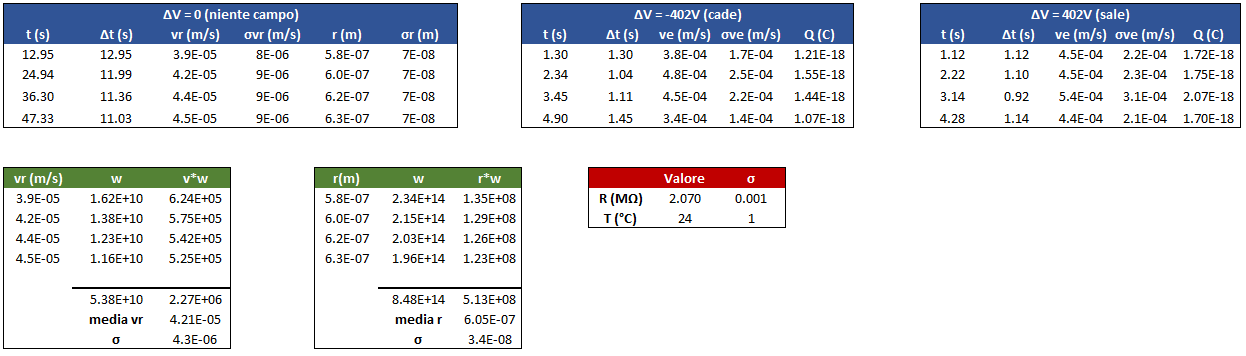
\includegraphics[width=\linewidth]{Goccia11}
\end{figure}

\pagebreak

Goccia 12:

\begin{figure}[h]
\centering
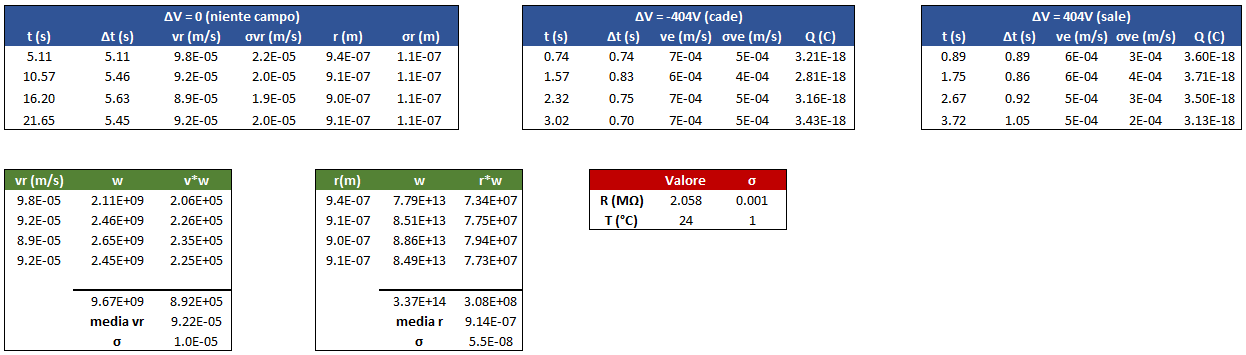
\includegraphics[width=\linewidth]{Goccia12}
\end{figure}

\vspace{10mm}

Goccia 13:

\begin{figure}[h]
\centering
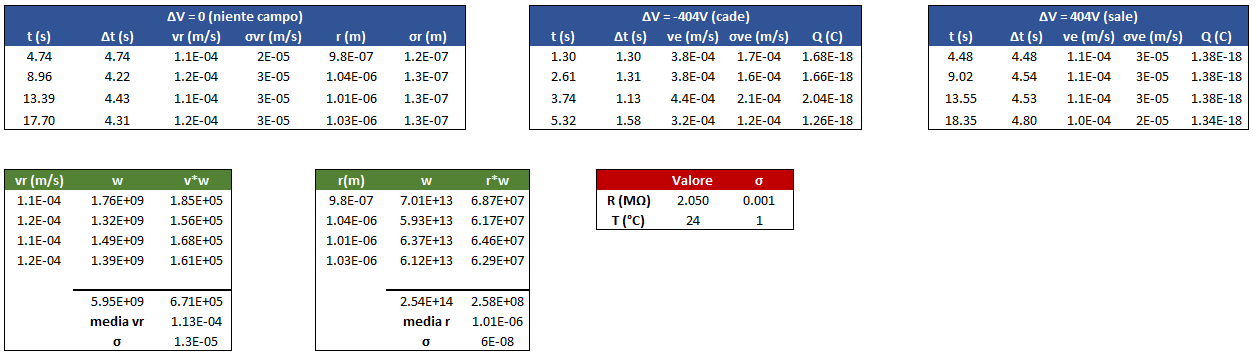
\includegraphics[width=\linewidth]{Goccia13}
\end{figure}

\vspace{10mm}

Goccia 14:

\begin{figure}[h]
\centering
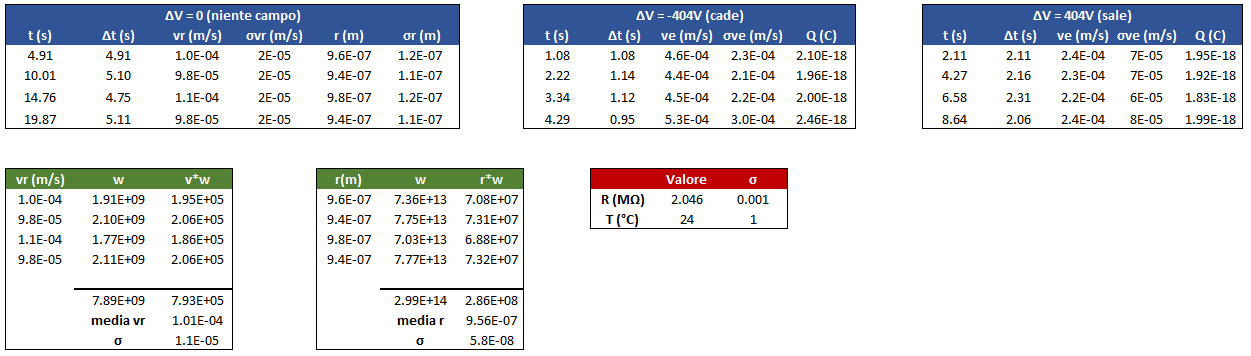
\includegraphics[width=\linewidth]{Goccia14}
\end{figure}

\pagebreak

Goccia 15:

\begin{figure}[h]
\centering
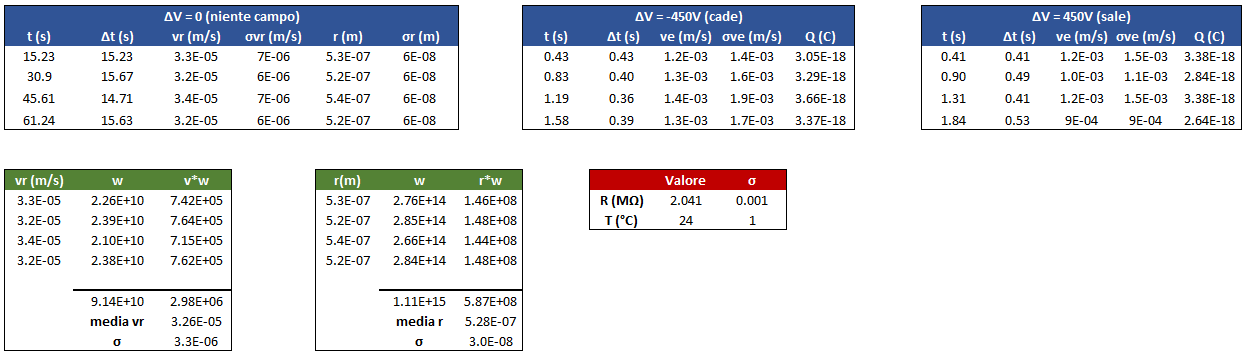
\includegraphics[width=\linewidth]{Goccia15}
\end{figure}

\vspace{10mm}

Goccia 16:

\begin{figure}[h]
\centering
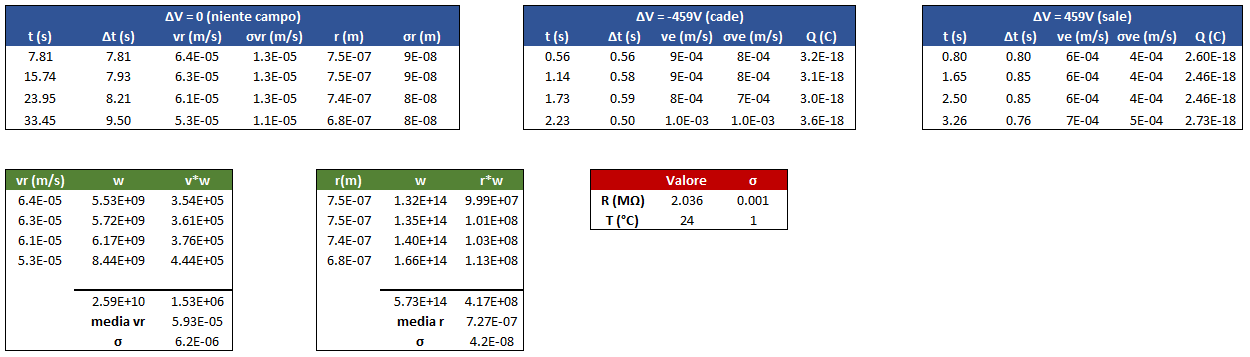
\includegraphics[width=\linewidth]{Goccia16}
\end{figure}

\vspace{10mm}

Goccia 17:

\begin{figure}[h]
\centering
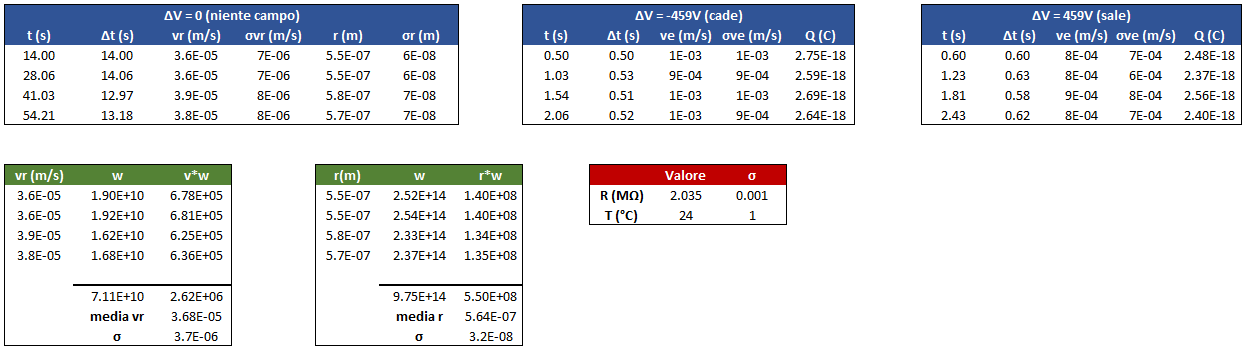
\includegraphics[width=\linewidth]{Goccia17}
\end{figure}

\pagebreak

Goccia 18:

\begin{figure}[h]
\centering
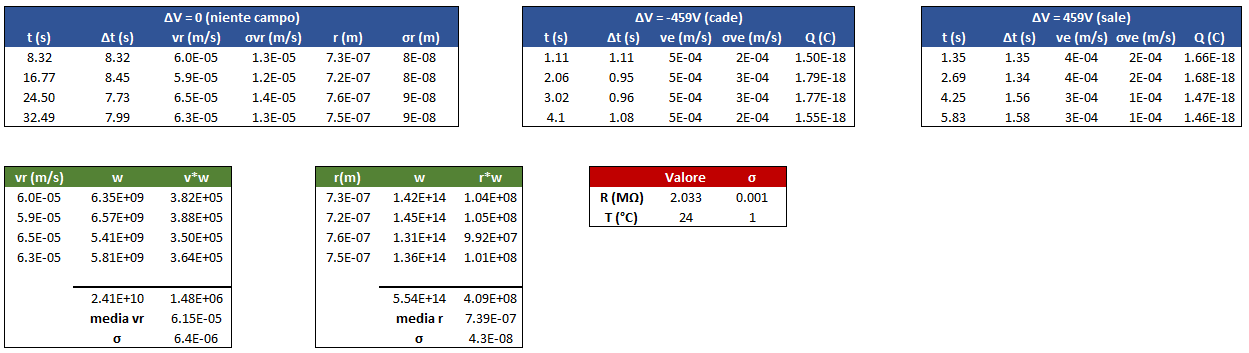
\includegraphics[width=\linewidth]{Goccia18}
\end{figure}

\vspace{10mm}

Goccia 19:

\begin{figure}[h]
\centering
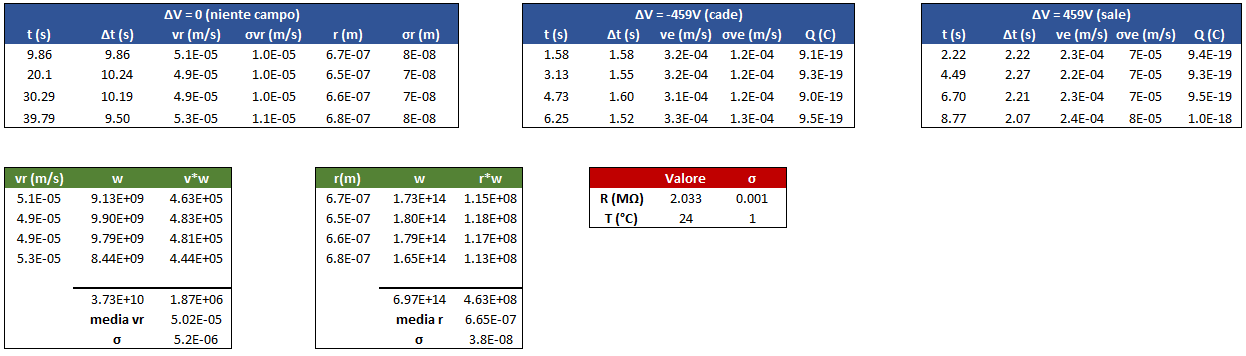
\includegraphics[width=\linewidth]{Goccia19}
\end{figure}

\subsection{Confronto raggi}

\begin{figure}[h]
\centering
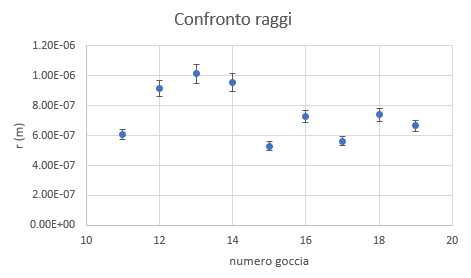
\includegraphics[width=0.6\linewidth]{Confronto_r_2}
\end{figure}

Le diverse gocce usate nell'esperimento hanno tutte raggi di dimensioni simili, ovvero dello stesso ordine di grandezza. Possiamo escludere l'eventualità di gravi errori nella presa dati.

Le dimensioni delle gocce sono tali da escludere effetti significativi di moti browniani.

\pagebreak

\section{Misure gocce 20-23}

I metodi e le analisi utilizzate nel secondo turno di laboratorio sono analoghe a quelle indicate per il primo. Le gocce trattate in questa sezione sono state misurate con l'apparato in dotazione a Alessandro Rossi, che dava i tempi ad Alessandro Matteo Rossi.

\vspace{5mm}

Problemi tecnici riscontrati: a causa della bassa responsività delle gocce, è stato fatto pesante uso della sorgente di Torio, che ha portato a gocce molto cariche. 

\subsection{Misura distanziale}

Sono state effettuate 5 misure dello spessore del distanziale

\begin{table}[h!]
\centering
\begin{tabular}{ | c | c | c | }
  \hline
  $\#$ & d (mm) & $\sigma$d (mm) \\
  \hline
  $1$ & $7,56$ & $0,01$ \\
  $2$ & $7,57$ & $0,01$ \\
  $3$ & $7,58$ & $0,01$ \\
  $4$ & $7,57$ & $0,01$ \\
  $5$ & $7,57$ & $0,01$ \\
  \hline
  & media & $\sigma$media \\
  \hline
  & $7,57$ & $0,01$ \\
  \hline
\end{tabular}
  \caption{Misura del distanziale}
  \label{dist_3}
\end{table}

come incertezza della media si è scelto di usare la sensibilità del micrometro.

\subsection{Misura delle gocce}

Goccia 20:

\begin{figure}[h]
\centering
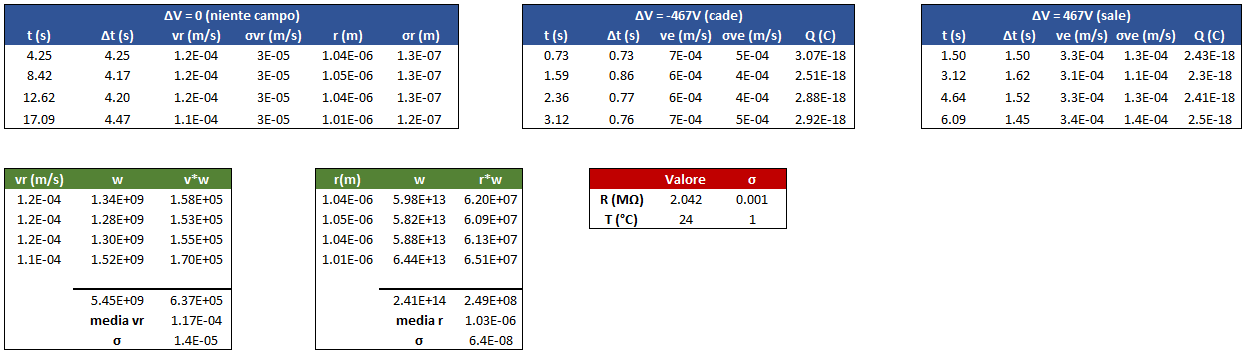
\includegraphics[width=\linewidth]{Goccia20}
\end{figure}

\pagebreak

Goccia 21:

\begin{figure}[h]
\centering
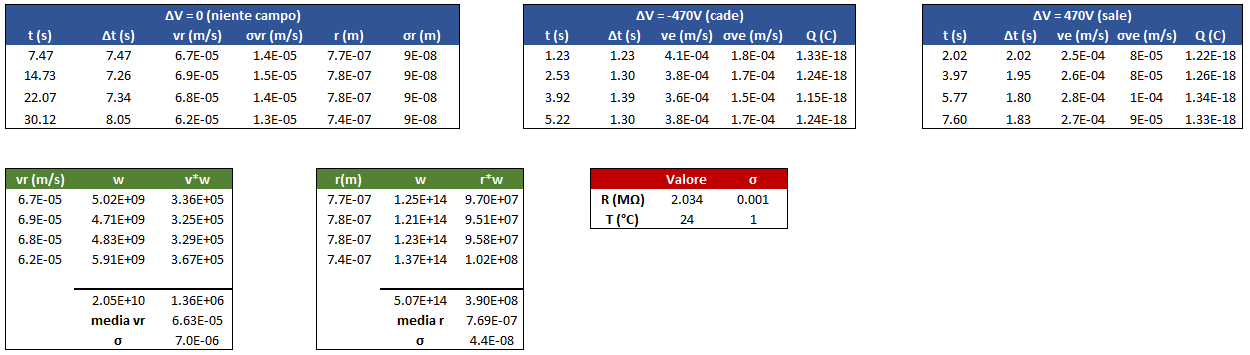
\includegraphics[width=\linewidth]{Goccia21}
\end{figure}

\vspace{10mm}

Goccia 22:

\begin{figure}[h]
\centering
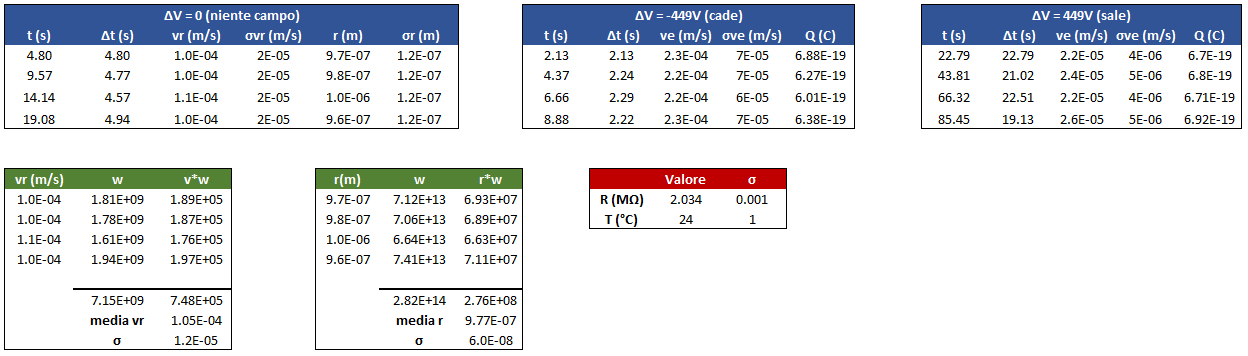
\includegraphics[width=\linewidth]{Goccia22}
\end{figure}

\vspace{10mm}

Goccia 23:

\begin{figure}[h]
\centering
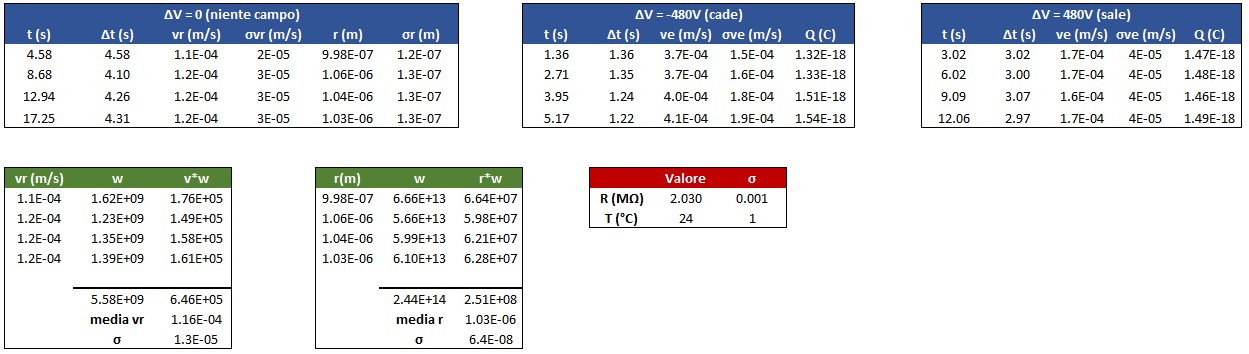
\includegraphics[width=\linewidth]{Goccia23}
\end{figure}

\pagebreak

\subsection{Confronto raggi}

\begin{figure}[h]
\centering
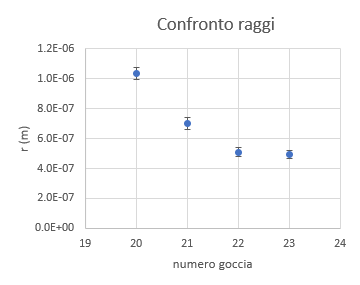
\includegraphics[width=0.5\linewidth]{Confronto_r_3}
\end{figure}

Le diverse gocce usate nell'esperimento hanno tutte raggi di dimensioni simili, ovvero dello stesso ordine di grandezza. Possiamo escludere l'eventualità di gravi errori nella presa dati.

Le dimensioni delle gocce sono tali da escludere effetti significativi di moti browniani.

\section{Analisi dei dati}

Sono state misurate 23 gocce, e per ciascuna di queste sono stati raccolte 4 misure della velocità. Per ogni misura abbiamo ricavato un valore di $Q$. In totale abbiamo quindi 184 misure di $Q$ da usare nella formula (\ref{Anal1}). Per l'analisi dei dati abbiamo scritto un programma in C++ che valuta la funzione S(q) tra $1,5 \cdot 10^{-19}$ C e $1,7 \cdot 10^{-19}$ C e la disegna usando ROOT. Abbiamo usato un passo di $0,002 \cdot 10^{-19}$ C, valutando quindi 101 punti differenti. Abbiamo ottenuto i seguenti risultati:

\begin{figure}[h]
\centering
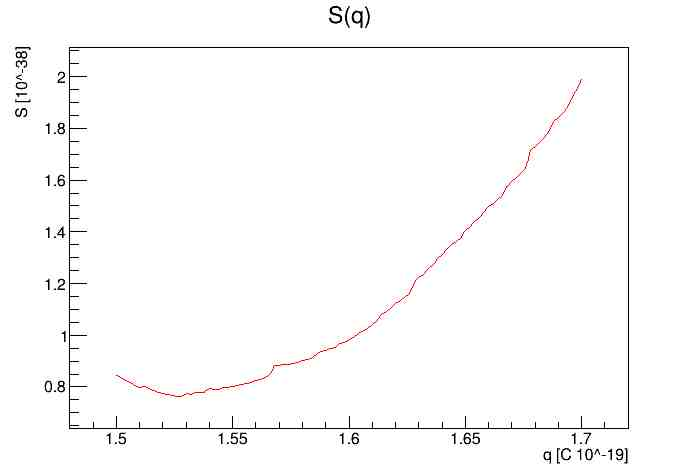
\includegraphics[width=0.8\linewidth]{Sq}
\caption{Grafico della funzione S(q), disegnato con ROOT}
\end{figure}

\[q_c = 1,526 \cdot 10^{-19} \textrm{C}\]

Abbiamo quindi implementato, nel programma, un ciclo per calcolare la media (\ref{Anal2}). Per evitare di entrare in una condizione di overflow abbiamo implementato un algoritmo iterativo per il calcolo della media

\[M_0 = 0\]
\[M_i = M_{i-1} + \frac{\frac{Q_i}{k_i(Q_i,q_c)} - M_{i-1}}{i}\]
\[M=M_N\]

E abbiamo fatto lo stesso per il calcolo della varianza

\[S_0 = 0\]
\[S_i = S_{i-1} + \frac{(\frac{Q_i}{k_i(Q_i,q_c)} - M)^2 - S_{i-1}}{i}\]
\[S=\sqrt{S_N}\]

La deviazione standard così ottenuta è l'incertezza della nostra misura $q_e$.

\[q_e = 1,52953 \cdot\ 10^{-19} \pm 6,41063 \cdot 10^{-21} \, \textrm{C}\]

Riducendo l'incertezza ad una cifra significativa e ricordando che la carica dell'elettrone ha segno negativo

\[q_e = - 1,53 \cdot\ 10^{-19} \pm 6 \cdot 10^{-21} \, \textrm{C}\]

Il valore accettato della carica dell'elettrone è 

\[q= - 1,6022 \cdot 10^{-19} \, \textrm{C}\]

\begin{figure}[h]
\centering
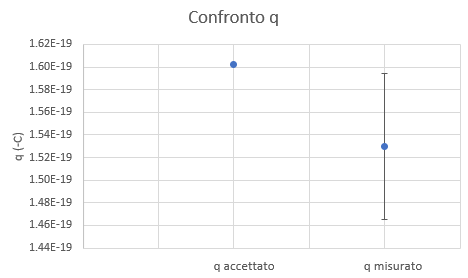
\includegraphics[width=0.7\linewidth]{Confronto_q}
\end{figure}

che dista il $4,5 \%$ dal valore $q_e$ misurato, in termini di deviazione standard dista $1,1 \sigma$. Il valore misurato può essere considerato accettabile, tuttavia, visto l'elevato numero di gocce misurate, sospettiamo la presenza di errori sistematici nelle nostre misure.

\vspace{5mm}

Ipotizziamo che la relativamente grande carica elettrica delle gocce 11-23 abbia portato ad un grafico di $S(q)$ più ''piatto'', rispetto al grafico relativo alle prime dieci gocce. Ricordando che 

\[\frac{Q_i}{k_i} - q = \frac{Q_i - qk_i}{k_i} \quad \textrm{dove} \quad 0 \leq \left|Q_i - qk_i\right| \leq q \quad \textrm{e} \quad \frac{q}{k_i} \quad \textrm{diminuisce al crescere di} \quad Q_i\]

segue che, nella computazione di $S(q)$, le gocce più cariche hanno minor peso delle gocce meno cariche. La nostra ipotesi è quindi che, unendo i dati raccolti nelle due sessioni di laboratorio, sia stato dato un peso significativamente maggiore alle gocce poco cariche raccolte nel primo turno di laboratorio. Abbiamo quindi rianalizzato i dati raccolti, questa volta separando le gocce raccolte nel primo turno di laboratorio (d'ora in poi chiameremo questo dataset $a$) da quelle raccolte nel secondo (dataset $b$).

\[q_{ca}=1,532 \quad q_a = 1,53 \cdot\ 10^{-19} \pm 8 \cdot 10^{-21} \, \textrm{C}\]

\[q_{cb}=1,608 \quad q_b = 1,61 \cdot\ 10^{-19} \pm 5 \cdot 10^{-21} \, \textrm{C}\]

\begin{figure}[h]
  \centering
  \begin{subfigure}[b]{0.4\linewidth}
    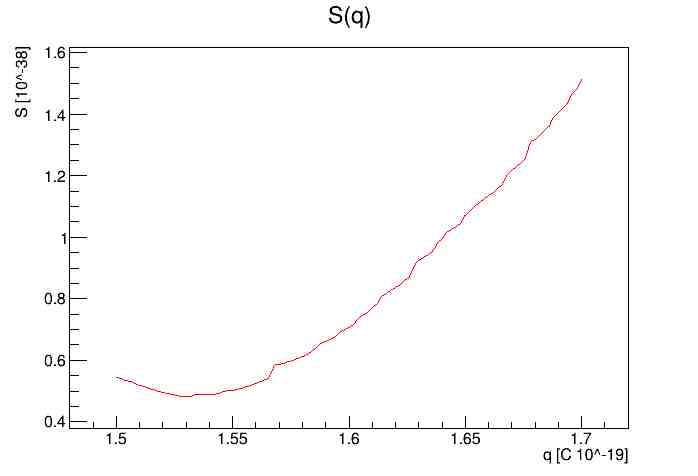
\includegraphics[width=\linewidth]{SA_q}
    \caption{Gocce 1-10}
  \end{subfigure}
  \begin{subfigure}[b]{0.4\linewidth}
    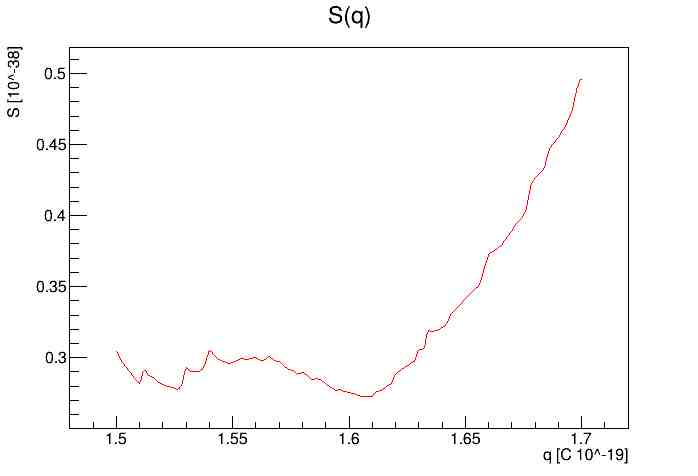
\includegraphics[width=\linewidth]{SB_q}
    \caption{Gocce 11-23}
  \end{subfigure}
\caption{Grafici di S(q) relativi ai due differenti set di dati a disposizione}
\label{rianalisi}
\end{figure}

L'analisi dei dati conferma la nostra ipotesi. Come visibile dai grafici in Figura \ref{rianalisi}, i valori della funzione $S_b(q)$ sono notevolmente più piccoli di quelli della funzione $S_a(q)$. Inoltre l'analisi del dataset $b$ fornisce un valore della carica dell'elettrone molto vicino al valore accettato, nentre l'analisi del dataset $a$ fornisce un valore in linea con la prima analisi. Siamo quindi sicuri che il valore ottenuto nella prima analisi sia dovuto al numero relativamente piccolo di dati raccolti nel primo turno di laboratorio, che giustifica un errore dell'ordine del $4\%$.

\vspace{5mm}

Abbiamo quindi deciso di scartare il valore di $q_e$ ottenuto dalla prima analisi e di usare, come miglior stima della carica dell'elettrone, la media pesata dei due valori $q_a$ e $q_b$ ottenuti da questa rianalisi, il cui valore è: 

\[q_e = 1,59 \cdot\ 10^{-19} \pm 4 \cdot 10^{-21} \, \textrm{C}\]

\pagebreak

\section{Conclusioni}

La nostra miglior stima della carica dell'elettrone è di 

\[q_e = - 1,59 \cdot\ 10^{-19} \pm 4 \cdot 10^{-21} \, \textrm{C}\]

\begin{figure}[h]
\centering
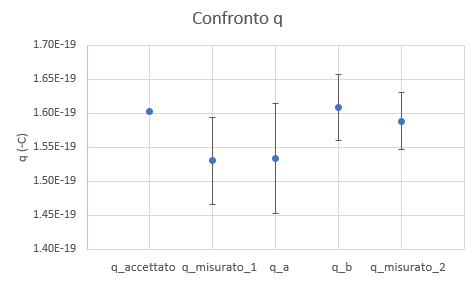
\includegraphics[width=0.7\linewidth]{Confronto_q_2}
\end{figure}

Perfettamente compatibile con il valore accettato.

\vspace{5mm}

L'esperimento può dirsi concluso con successo.

\end{document}